\subsection{p53 DNA Damage Repair}

\begin{frame}

  \frametitle{p53 ``Guardian of the Cell''}

  \begin{itemize}
  \item Responsible for Repairing DNA damage
  \item Activates DNA Repair proteins
  \item Pauses the Cell Cycle (prevents replication of damage DNA)
  \item Initiates \emph{apoptosis} (cell death) in the case where damage can't
    be repaired.
  \item Large scale feeback loop with NF-$\kappa$B\textbf{.}
  \end{itemize}

\end{frame}


\begin{frame}
  \frametitle{p53 DNA Damage Repair}

  % 
  \begin{figure}
    \includegraphics[width=0.45\textwidth]{../../../sysbio/tex/diagrams/p53-unbound}\hfill{}\includegraphics[width=0.4\textwidth]{../../../sysbio/tex/diagrams/p53-bound}

    \caption{p53. \emph{Left} unbound, \emph{Right }bound to DNA. Images by David
      S. Goodsell from \protect\url{http://www.rcsb.org/} (see the {}``Molecule
      of the Month'' feature).}

  \end{figure}



\end{frame}


\begin{frame}
  \frametitle{p53}

  % 
  \begin{figure}
    \begin{centering}
      \includegraphics[angle=90,width=0.6\textwidth]{../../../sysbio/tex/diagrams/f013802.jpeg}
      \par\end{centering}

    \caption{Repair of DNA damage by p53. Image from\citet{Goodsell:p53tumor99}.}

  \end{figure}

\end{frame}


\begin{frame}
  \frametitle{Modelling Assumption}
  \begin{itemize}
  \item Assume p53 affects targets as a single input module network motif
    (SIM).
  \end{itemize}
  % 
  \begin{figure}
    \begin{centering}
      \includegraphics[width=0.4\textwidth]{../../../sysbio/tex/diagrams/p53_sim}
      \par\end{centering}

    \caption{p53 SIM network motif as modelled by \citealt{Barenco:ranked06}.}

  \end{figure}



\end{frame}


\begin{frame}
  \frametitle{p53 (RBF covariance)}

  \begin{flushright}
    \textbf{Pei Gao}
    \par\end{flushright}

  % 
  \begin{figure}
    \centering{} 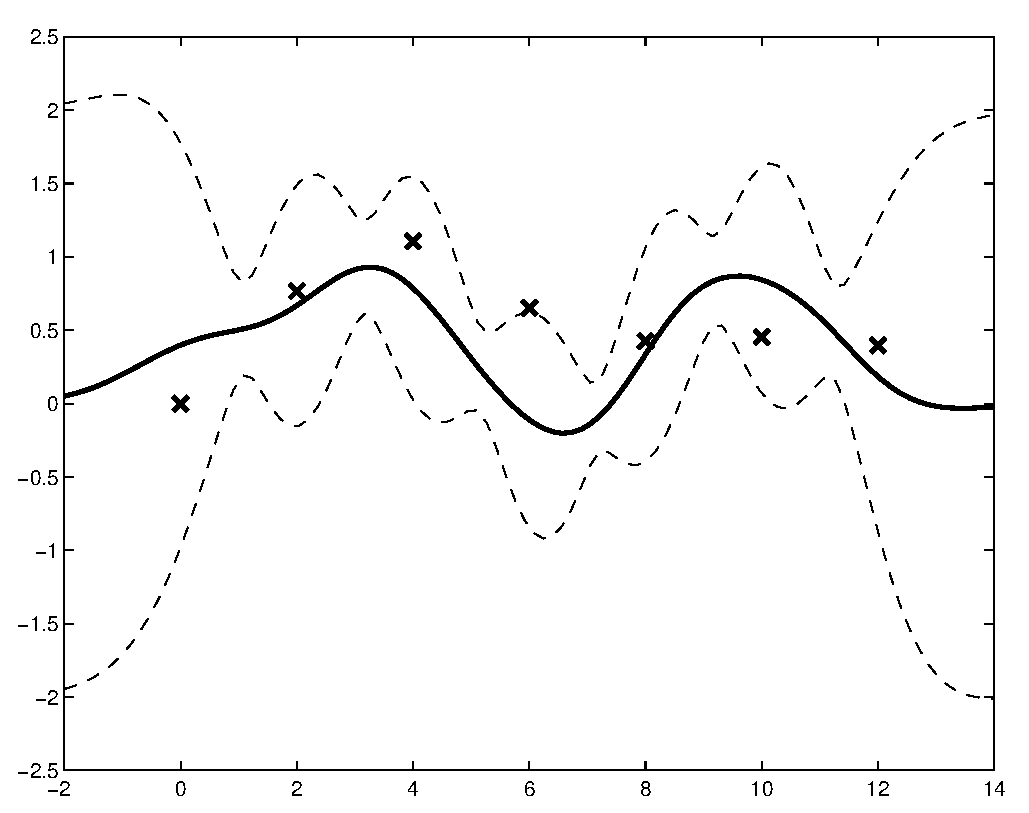
\includegraphics[width=0.3\textwidth]{../../../gpsim/tex/diagrams/demBarenco1_profile2}
    \hfill{}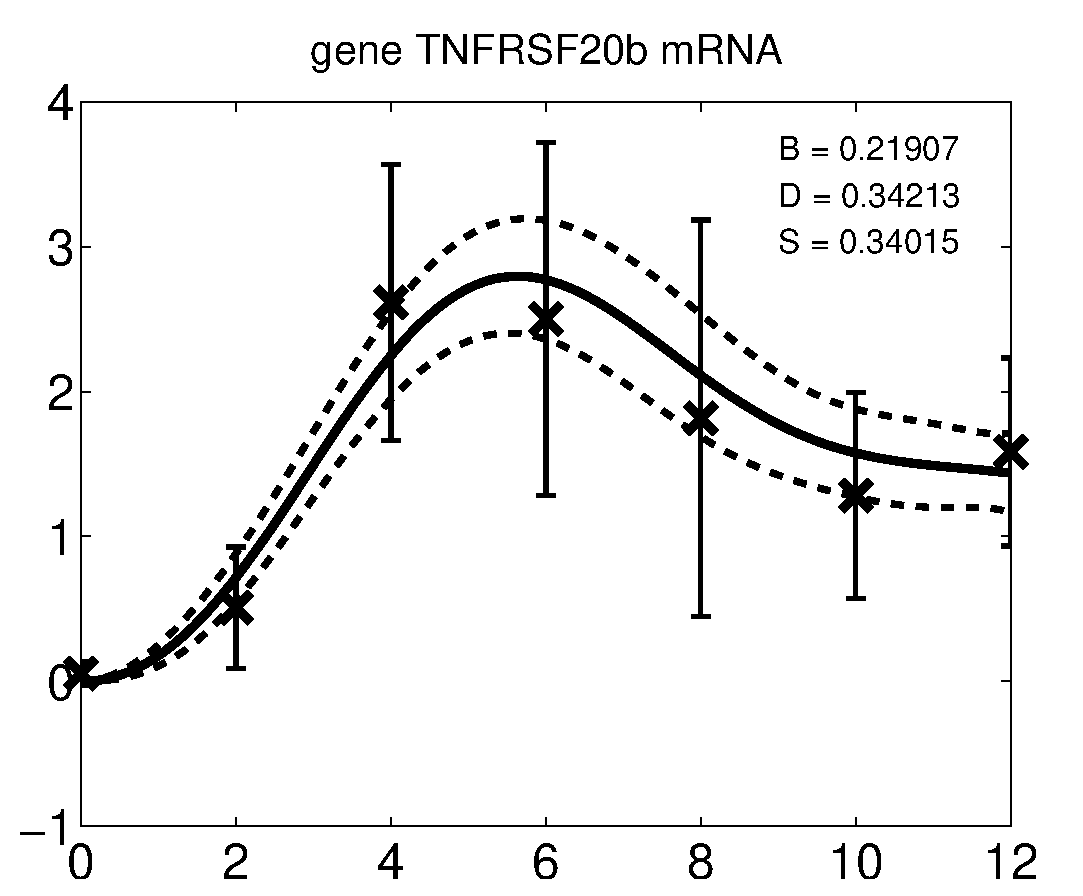
\includegraphics[width=0.3\textwidth]{../../../gpsim/tex/diagrams/demBarenco1_ExprsProfile_Rep2_Gene3}\hfill{}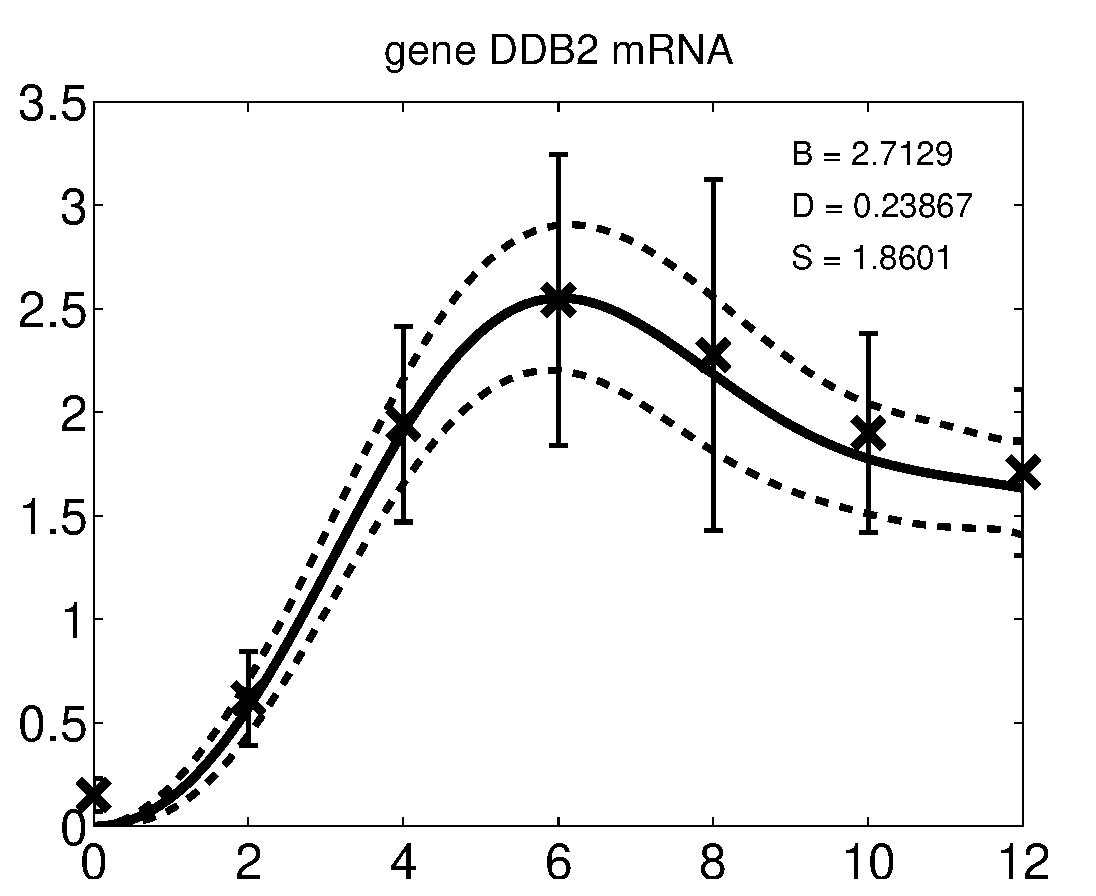
\includegraphics[width=0.3\textwidth]{../../../gpsim/tex/diagrams/demBarenco1_ExprsProfile_Rep2_Gene1}\\
    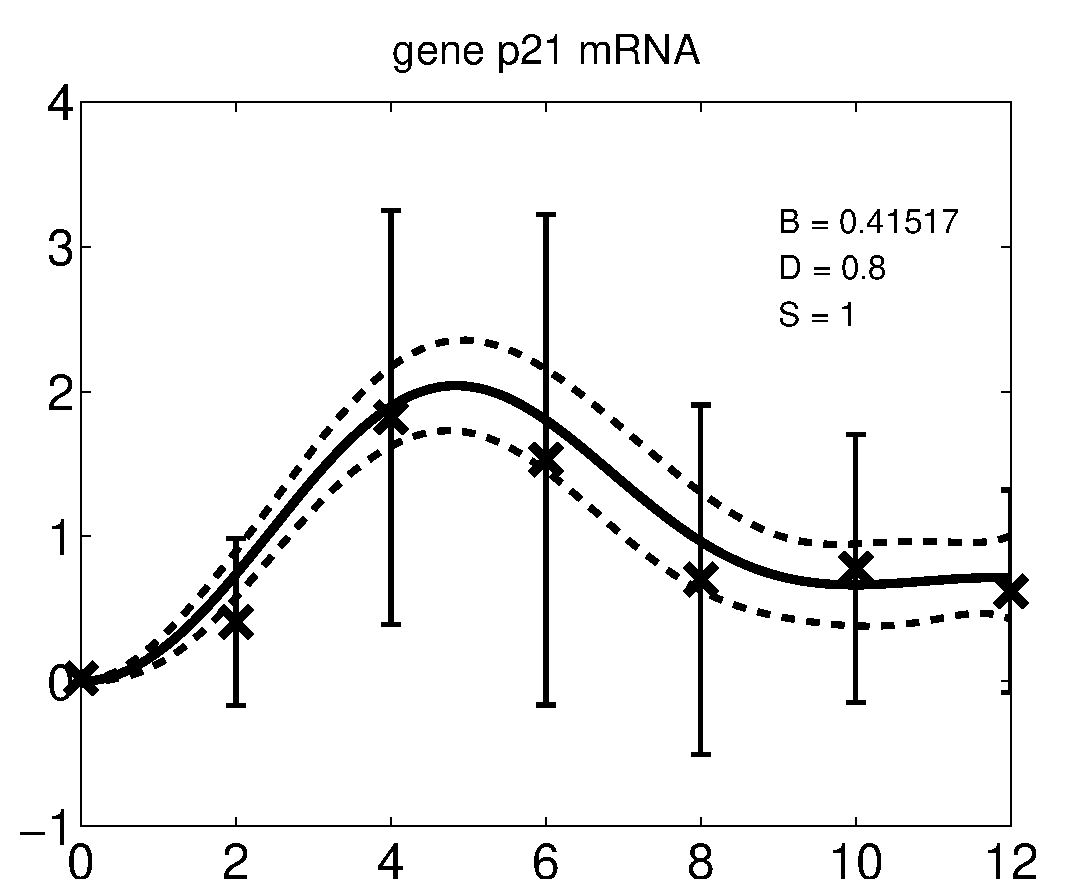
\includegraphics[width=0.3\textwidth]{../../../gpsim/tex/diagrams/demBarenco1_ExprsProfile_Rep2_Gene4}
    \hfill{}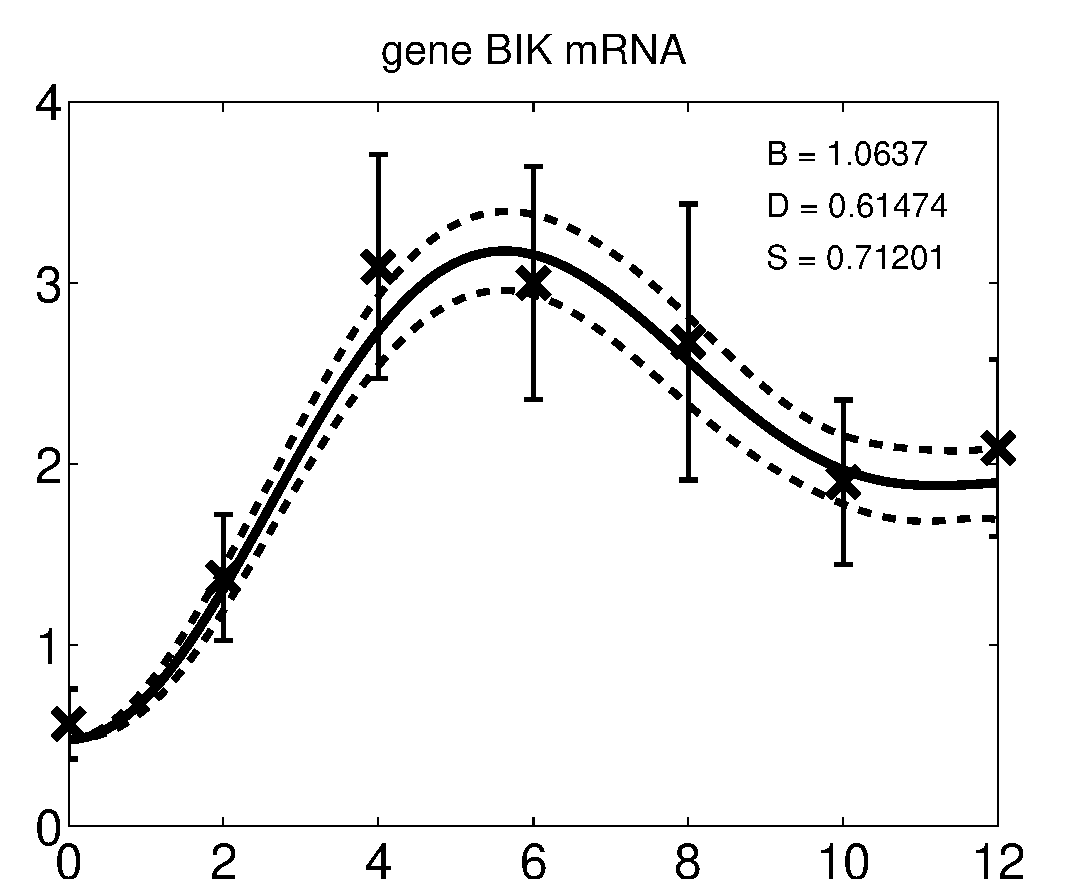
\includegraphics[width=0.3\textwidth]{../../../gpsim/tex/diagrams/demBarenco1_ExprsProfile_Rep2_Gene2}
    \hfill{}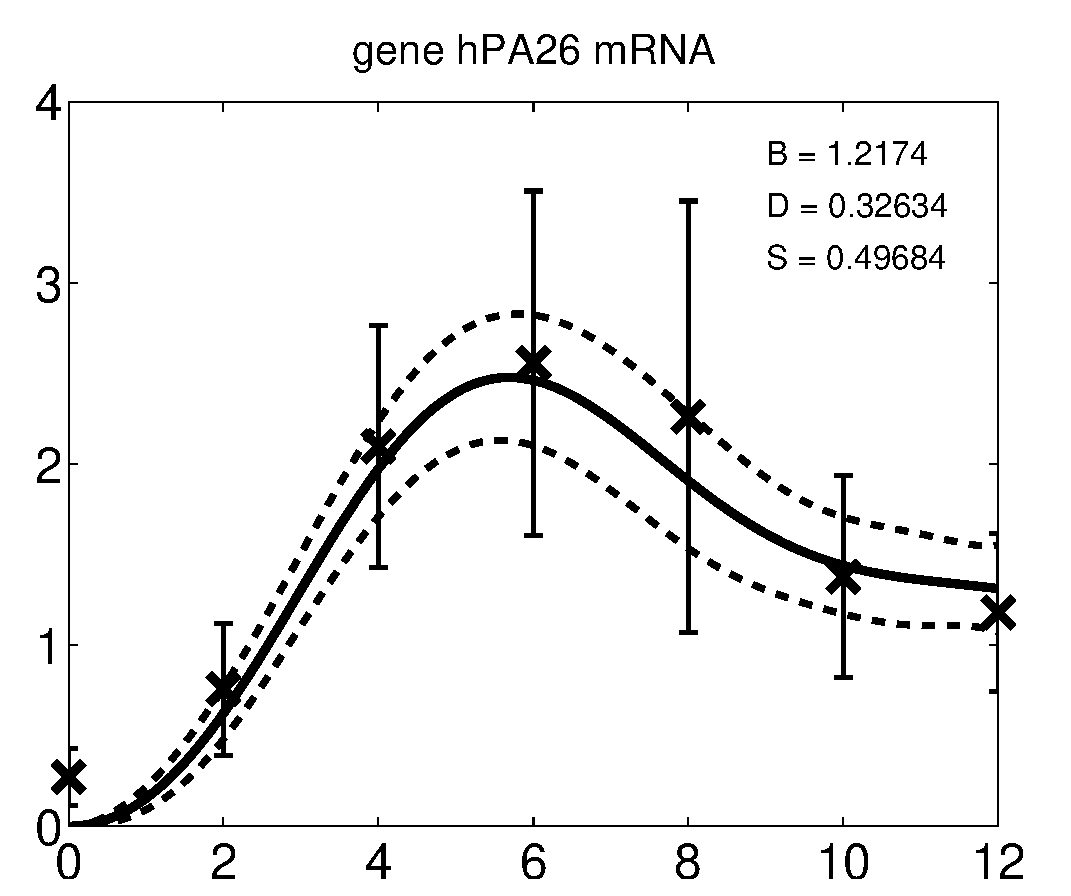
\includegraphics[width=0.3\textwidth]{../../../gpsim/tex/diagrams/demBarenco1_ExprsProfile_Rep2_Gene5} 
  \end{figure}



\end{frame}

